\section{Misura di C\textsubscript{D} al banco prova} \label{sez:cd}

\subsection{Presentazione del banco prova, dati e richieste}
Viene realizzato un banco prova per misure di temperatura mediante termocoppia. Tale banco è alimentato da gas naturale, che passa per un misuratore di portata a galleggiante, raggiunge una camera di stanca dove se ne misura la temperatura, poi viene accelerato da un ugello in un eiettore, che fornisce la portata d'aria per permettere la combustione. Un misuratore di pressione differenziale è inserito tra camera di stanca e ambiente esterno. Infine la miscela è combusta in un bruciatore. Lo schema completo del banco prova è consultabile in App.\ref{app:banco}. 

Si richiede di misurare il coefficiente di efflusso (\gls{symb:cd}) dell'ugello utilizzando le misure a disposizione, di studiare l'andamento rispetto alla portata reale e al variare della pressione differenziale; infine, studiare l'andamento al variare di \gls{symb:ma} e \gls{symb:re}.

Gli strumenti di misura a disposizione sono i seguenti:
\begin{itemize}
	\item Misuratore di portata a galleggiante con scala graduata in Nl/min (condizioni normali $T_N$ = 273 K, $P_N$ = 1 atm);
	\item Barometro differenziale digitale in mbar;
	\item Termometro digitale in \textsuperscript{o}C.
\end{itemize}

Il diametro dell'ugello (\gls{symb:Du}) è pari a 2.7 mm. La pressione ambiente (\gls{symb:pamb}) ammonta a 100600 Pa al momento della misura.

La procedura per definire \gls{symb:cd} parte dalla definizione del coefficiente di efflusso:
\begin{equation}
	C_D=\frac{\dot{m}_\textit{REALE}}{\dot{m}_\textit{TEORICA}}
\end{equation}
dove $\dot{m}_\textit{REALE} = q_M$, mentre $\dot{m}_\textit{TEORICA}$ viene ottenuta mediante alcune assunzioni. 

Per quanto riguarda $q_M$, essa è ottenuta dalla portata misurata mediante galleggiante usando $q_M=q_{MN} \rho_N$.

Per il calcolo di \gls{symb:mdot}\textsubscript{\textit{TEORICA}} è possibile utilizzare il teorema di Bernoulli e determinare \gls{symb:V}\textsubscript{\textit{TEORICA}} mediante: 
\begin{equation}
	V_{\textit{TEORICA}} = \sqrt{\frac{2\Delta p}{\rho}} \label{eq:velocità}
\end{equation}
per poi trovare \gls{symb:mdot}\textsubscript{\textit{TEORICA}} mediante:
\begin{equation}
	\dot{m}_{\textit{TEORICA}}=\rho	V_{\textit{TEORICA}} A \label{eq:portata}
\end{equation}


\paragraph{Ipotesi}
Lo svolgimento della misura richiede l'assunzione di alcune ipotesi, alcune delle quali sono poi verificate a seguito della misura stessa. 

\begin{itemize}
	\item Assunzione di profilo di velocità uniforme nella sezione di efflusso.
	\item Effetti di viscosità trascurabili e flusso incomprimibile (per la validità del teorema di Bernoulli): tale ipotesi permette di assumere che \gls{symb:T} sia costante nel flusso e che l'ugello scarichi a \gls{symb:pamb}. 
	\item Gas naturale considerabile come puro metano, nonché come gas perfetto.
\end{itemize}

\subsection{Presentazione dei valori misurati}
A seguito delle misure sono rilevati i valori riportati in Tab.\ref{tab:dati}, a cui è associata la conversione nelle unità di misura opportune. In particolare, per convertire $q_{NM}$ in $q_M$ si utilizza la seguente relazione: $q_M=q_{NM} \rho_N /6e4$, dove 6e4 è un fattore di conversione per passare da Nl/min a kg/s, mentre $\rho_N$ è ottenuto a 1 atm e 273 K tramite $\rho_N = p/(RT) = 0.7142$ kg/m\textsuperscript{3}. Il valore di \gls{symb:R} è pari a quello per il metano, che ammonta a 520 J/(kgK).

\begin{table}[H]
	\centering
	\begin{tabular}{c|c|c|c|c|c|c}
		\toprule
		\toprule
		\textbf{Misura}& \textbf{q\textsubscript{MN} [Nl/min]}  & \textbf{q\textsubscript{M} [kg/s]}& \textbf{$\Delta$p [mbar]}  & \textbf{$\Delta$p [Pa]} & \textbf{T [°C]}  & \textbf{T [K] } \\
	\midrule
	\midrule
1  & 7  &8.33e-05 	& 0.5 & 50   & 32.1 & 305.1 \\
		\midrule
		2  & 9  &1.07e-04& 1.8 & 180  & 32.1 & 305.1 \\\midrule
		3  & 10 &1.19e-04& 3.6 & 360  & 32.0   & 305.0   \\\midrule
		4  & 11 &1.31e-04& 4.4 & 440  & 31.9 & 304.9 \\\midrule
		5  & 12 &1.43e-04& 5.5 & 550  & 31.8 & 304.8 \\\midrule
		6  & 14 &1.67e-04& 7.8 & 780  & 31.7 & 304.7 \\\midrule
		7  & 15 &1.79e-04& 9.5 & 950  & 31.7 & 304.7 \\\midrule
		8  & 16 &1.90e-04& 11.3 & 1130 & 31.6 & 304.6 \\\midrule
		9  & 17 &2.02e-04& 12.8 & 1280 & 31.6 & 304.6 \\\midrule
		10 & 18 &2.14e-04& 14.2 & 1420 & 31.5 & 304.5 \\\midrule
		11 & 19 &2.26e-04& 15.9 & 1590 & 31.5 & 304.5 \\\midrule
		12 & 20 &2.38e-04& 17.5 & 1750 & 31.5 & 304.5 \\
		\bottomrule
		\bottomrule
	\end{tabular}
	\caption{Grandezze misurate e conversioni}
	\label{tab:dati}
\end{table}

Successivamente vengono calcolate le seguenti quantità:
\begin{itemize}
	\item \gls{symb:rho} mediante l'ipotesi di gas perfetto ($\rho = p/(RT)$); il valore di \gls{symb:p} è ottenuto tramite $p=p_{\textit{AMB}}+\Delta p$, questa relazione è valida in quanto l'ugello scarica il flusso esattamente a pressione ambiente. 
	\item \gls{symb:V}\textsubscript{\textit{TEORICA}} mediante Eq.(\ref{eq:velocità}).
	\item \gls{symb:mdot}\textsubscript{\textit{TEORICA}} tramite Eq.(\ref{eq:portata}).
\end{itemize}


\begin{table}[H]
	\centering
	\begin{tabular}{c|c|c|c}
		\toprule
		\toprule
		\textbf{Misura} & \textbf{$\bm{\rho}$ [kg/m\textsuperscript{3}]} & \textbf{V\textsubscript{\textit{TEORICA}} [m/s]} 
		& \textbf{$\bm{\dot{m}}$ [kg/s]}  \\
		\midrule
		\midrule
		1 & 0.635 & 12.6 & 4.56e-05 \\
		\midrule
		2 & 0.636 & 23.8 & 8.66e-05 \\
		\midrule
		3 & 0.637 & 33.6 & 1.23e-04 \\
		\midrule
		4 & 0.638 & 37.1 & 1.36e-04 \\
		\midrule
		5 & 0.639 & 41.5 & 1.52e-04 \\
		\midrule
		6 & 0.640 & 49.4 & 1.81e-04 \\
		\midrule
		7 & 0.641 & 54.4 & 2.00e-04 \\
		\midrule
		8 & 0.643 & 59.3 & 2.18e-04 \\
		\midrule
		9 & 0.644 & 63.1 & 2.32e-04 \\
		\midrule
		10 & 0.645 & 66.4 & 2.45e-04 \\
		\midrule
		11 & 0.646 & 70.2 & 2.59e-04 \\
		\midrule
		12 & 0.647 & 73.6 & 2.72e-04 \\
		\bottomrule
		\bottomrule
	\end{tabular}
	\caption{Calcoli intermedi}
	\label{tab:calcoli_intermedi}
\end{table}

Da questi valori è possibile ottenere una stima del valore di \gls{symb:cd} per ciascuna misura. Si presentano anche i grafici che rappresentano la dipendenza di \gls{symb:cd} dalle tre misure al fine di evidenziare eventuali dipendenze ed errori.
\begin{table}[H]
	\centering
	\begin{tabular}{c|c}
		\toprule
		\toprule
		\textbf{Misura} & \textbf{C\textsubscript{D}} \\
		\midrule
		\midrule
		1  & 1.827 \\
		\midrule
		2  & 1.237 \\
		\midrule
		3  & 0.971 \\
		\midrule
		4  & 0.965 \\
		\midrule
		5  & 0.941 \\
		\midrule
		6  & 0.921 \\
		\midrule
		7  & 0.893 \\
		\midrule
		8  & 0.873 \\
		\midrule
		9  & 0.871 \\
		\midrule
		10 & 0.875 \\
		\midrule
		11 & 0.872 \\
		\midrule
		12 & 0.874 \\
		\bottomrule
		\bottomrule
	\end{tabular}
	\caption{Valori di C\textsubscript{D} per ciascuna misura}
	\label{tab:valori_cd}
\end{table}
\begin{figure}
	\centering
	\includegraphics[width=0.5\linewidth]{"chapters/5-laboratorio/tabellaqmcd"}
	\caption{Dipendenza di \gls{symb:cd} da $q_M$}
	\label{fig:tabellaqmcd}
\end{figure}
\begin{figure}
	\centering
	\includegraphics[width=0.5\linewidth]{"chapters/5-laboratorio/tabelladeltapcd"}
	\caption{Dipendenza di \gls{symb:cd} da $\Delta p$}
	\label{fig:tabelladeltapcd}
\end{figure}

\begin{figure}
	\centering
	\includegraphics[width=0.5\linewidth]{"chapters/5-laboratorio/tabellaTcd"}
	\caption{Dipendenza di \gls{symb:cd} da \gls{symb:T}}
	\label{fig:tabellatcd}
\end{figure}
Da Fig.\ref{fig:tabellaqmcd}, così come da Fig.\ref{fig:tabelladeltapcd}, si osserva che le prime due misure risultano affette da errore significativo, il quale porta a ottenere valori di \gls{symb:cd} maggiori di 1 che non hanno significato fisico. Si osserva anche che la stima di \gls{symb:cd} si assesta attorno a 0.87 a partire dalla settima misura. Tale valore viene assunto come una stima ragionevole per \gls{symb:cd}.

Si nota anche che l'utilizzo di una pressione ambiente non standard ha un impatto limitato in quanto non porta a variazioni significative di \gls{symb:cd}: in media, avere \gls{symb:pamb} pari a 1 atm porta a un decremento di circa 0.35 \%.

Infine, la variazione di \gls{symb:T} misurata non porta a variazioni significative di \gls{symb:cd}. Gli unici valori anomali corrispondono alle prime due misure, affette da significativo errore. 

\subsection{Dipendenza da Reynolds e Mach}
Si riportano dei grafici rappresentanti la dipendenza di \gls{symb:cd} dal numero di Reynolds (Fig.\ref{fig:dipendenzare}) e dal numero di Mach (Fig.\ref{fig:dipendenzama}). 
Al fine di calcolare il valore di \gls{symb:mu} al variare di \gls{symb:T} viene utilizzata la legge di Sutherland:
\begin{equation}
	\mu = \mu_{\textit{REF}} \left( \frac{T}{T_{\textit{REF}}} \right)^{1.5} \frac{T_{\textit{REF}}+S}{T+S}
\end{equation}
Mediante $\mu_{\textit{REF}}$ = 1.03e-5 Pa\,s, $T_{\textit{REF}}$ = 273 K e $\mu_{\textit{100}}$ = 1.37e-5 Pa\,s a $T$ = 373 K si calcola \gls{symb:S} per il metano.
Infine si calcola \gls{symb:mu} al variare della temperatura. 
La variazione di \gls{symb:mu} è molto limitata in quanto \gls{symb:T} mantiene approssimativamente lo stesso valore per tutte le misure. 
Per il calcolo di \gls{symb:ma} si utilizza \gls{symb:gamma} pari a 1.3 al fine di calcolare la velocità del suono locale. 

\begin{figure}[H]
	\centering
	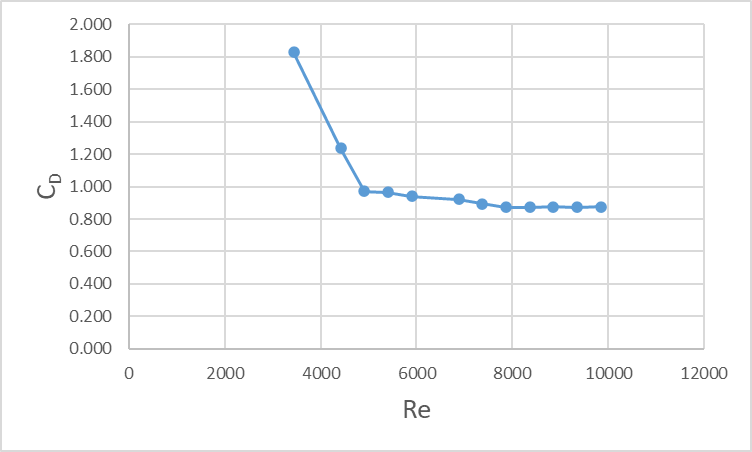
\includegraphics[width=0.7\linewidth]{chapters/5-laboratorio/dipendenzaRe2}
		\caption{Dipendenza di \gls{symb:cd} da \gls{symb:re}}
	\label{fig:dipendenzare}
\end{figure}

\begin{figure}[H]
	\centering
	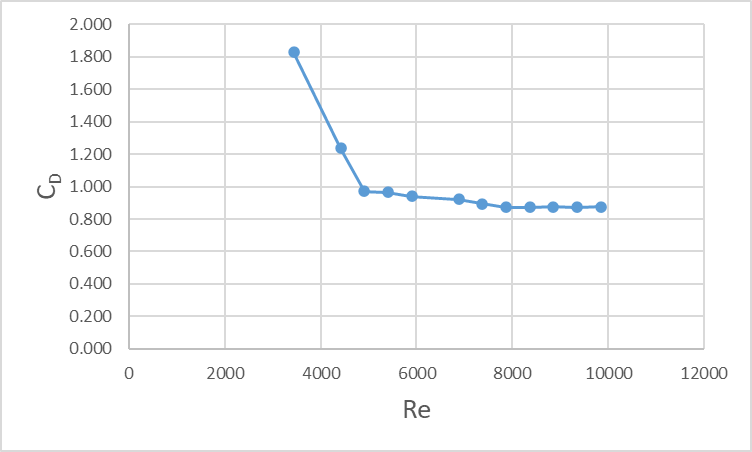
\includegraphics[width=0.7\linewidth]{chapters/5-laboratorio/dipendenzaMa2}
	\caption{Dipendenza di \gls{symb:cd} da \gls{symb:ma}}
	\label{fig:dipendenzama}
\end{figure}




Dai grafici è possibile osservare che: 
\begin{itemize}
	\item i primi valori di \gls{symb:cd} non sono significativi;
	\item \gls{symb:re} varia tra 3000 e 9000; ne deriva che il flusso nell'ugello è turbolento e valgono le ipotesi di profilo di velocità uniforme e di assenza di effetti viscosi significativi;
	\item \gls{symb:ma} è sempre ridotto, pertanto vale l'ipotesi di flusso incomprimibile: di conseguenza le perdite legate al ristagno del flusso sulla termocoppia sono considerate trascurabili. 
\end{itemize}
